\documentclass[
  parskip=half,           % halbzeiliger Zeileneinzug nach Absatz
  bibliography=totoc,     % Literatur im Inhaltsverzeichnis
  captions=tableheading,  % Tabellenüberschriften
  titlepage=firstiscover, % Titelseite ist Deckblatt
]{scrartcl}

\usepackage{geometry}
\geometry{a4paper,left=25mm,right=25mm, top=3cm, bottom=3cm}

% Paket float verbessern
\usepackage{scrhack}

% Warnung, falls nochmal kompiliert werden muss
\usepackage[aux]{rerunfilecheck}

% deutsche Spracheinstellungen
\usepackage{polyglossia}
\setmainlanguage{german}

% unverzichtbare Mathe-Befehle
\usepackage{amsmath}
% viele Mathe-Symbole
\usepackage{amssymb}
% Erweiterungen für amsmath
\usepackage{mathtools}

% Fonteinstellungen
\usepackage{fontspec}
% Latin Modern Fonts werden automatisch geladen

\usepackage[
  math-style=ISO,    % ┐
  bold-style=ISO,    % │
  sans-style=italic, % │ ISO-Standard folgen
  nabla=upright,     % │
  partial=upright,   % ┘
  warnings-off={           % ┐
    mathtools-colon,       % │ unnötige Warnungen ausschalten
    mathtools-overbracket, % │
  },                       % ┘
]{unicode-math}

% traditionelle Fonts für Mathematik
\setmathfont{Latin Modern Math}
\setmathfont{XITS Math}[range={scr, bfscr}]
\setmathfont{XITS Math}[range={cal, bfcal}, StylisticSet=1]

% Zahlen und Einheiten
\usepackage[
  locale=DE,                 % deutsche Einstellungen
  separate-uncertainty=true, % immer Fehler mit \pm
  per-mode=reciprocal,       % ^-1 für inverse Einheiten
  % alternativ:
  % per-mode=reciprocal, % m s^{-1}
  % decimal-marker=., % . statt , f�r Dezimalzahlen
]{siunitx}

% chemische Formeln
\usepackage[
  version=4,
  math-greek=default, % ┐ mit unicode-math zusammenarbeiten
  text-greek=default, % ┘
]{mhchem}

% tikzpicture ("Zeichenprogramm")
\usepackage{tikz}
\usetikzlibrary{circuits.ee.IEC}
\usetikzlibrary{positioning}
\tikzset{
  Pfeil/.style={thick,shorten >=#1,shorten <=#1,->,>=latex}, % für Peile
  UPfeil/.style={blue,Pfeil=#1,font={\sffamily\itshape}},% für Spannungspfeile
  IPfeil/.style={red,Pfeil=#1,font={\ttfamily\itshape}} % für Strompfeile
}
%Volt- und Amperemeter festlegen:
\tikzset{circuit declare symbol = Us}
\tikzset{set Us graphic ={draw,generic circle IEC, minimum size=5mm,info=center:$U_s$}}

\tikzset{circuit declare symbol = voltmeter}
\tikzset{set voltmeter graphic ={draw,generic circle IEC, minimum size=5mm,info=center:V}}

% richtige Anführungszeichen
\usepackage[autostyle]{csquotes}

% schöne Brüche im Text
\usepackage{xfrac}

\usepackage{blindtext}    % \blindtext zum Testen von Texten.

% Standardplatzierung für Floats einstellen
\usepackage{float}
\floatplacement{figure}{htbp}
\floatplacement{table}{htbp}

% Floats innerhalb einer Section halten
\usepackage[
  section, % Floats innerhalb der Section halten
  below,   % unterhalb der Section aber auf der selben Seite ist ok
]{placeins}

% Seite drehen für breite Tabellen
\usepackage{pdflscape}

% mehrere Seiten einer einzelnen pdf, zB
% \includepdf[pages={1-2}]{Bilder/Messdaten.pdf}
\usepackage{pdfpages}

% Captions schöner machen.
\usepackage[
  labelfont=bf,        % Tabelle x: Abbildung y: ist jetzt fett
  font=small,          % Schrift etwas kleiner als Dokument
  width=0.9\textwidth, % maximale Breite einer Caption schmaler
  %indention=1cm        % Einrückung nach der ersten Zeile
]{caption}
% subfigure, subtable, subref
\usepackage{subcaption}

% mit Buchstabend gelistete items: \begin{enumerate}[label={\alph*)}]
\usepackage{enumitem}

% Grafiken können eingebunden werden
\usepackage{graphicx}
% größere Variation von Dateinamen möglich (Probleme mit Leerzeichen behoben)
\usepackage{grffile}

% schöne Tabellen
\usepackage{booktabs}
\sisetup{table-format=1.2}
%\begin{tabular}{S[table-format=3.0] S S S S[table-format=3.2]}
%table-format : 3 stellen vor, 0 stellen nach dem Komma
% S steht f�r siunix, dh. wir verwenden solche Zahlen
% \multicolumn{2}{c}{Spalte 1}
% wie in excel Spalten zusammenf�gen
% Einheiten: {$\lambda \:/\: \si{\nano\meter}$}

% Uncertainties:
%\begin{tabular}{
% S[table-format=3.1]
% @{${}\pm{}$}
% S[table-format=2.1]
% }
% \toprule
% \multicolumn{2}{c}{$x \:/\: \si{\ohm}$} \\
% \midrule
% 632.4 & 5.7 \\

% Verbesserungen am Schriftbild
\usepackage{microtype}

% Literaturverzeichnis
\usepackage[
  backend=biber,
]{biblatex}
% Quellendatenbank
\addbibresource{Quellen.bib}
\addbibresource{programme.bib}

% Hyperlinks im Dokument
\usepackage[
  unicode,        % Unicode in PDF-Attributen erlauben
  pdfusetitle,    % Titel, Autoren und Datum als PDF-Attribute
  pdfcreator={},  % ┐ PDF-Attribute säubern
  pdfproducer={}, % ┘
  linkcolor=blue, % einfache interne Verkn?pfungen
  citecolor=blue, % Verweise auf Literaturverzeichniseintr?ge im Text
]{hyperref}
% erweiterte Bookmarks im PDF
\usepackage{bookmark}

% Trennung von Wörtern mit Strichen
\usepackage[shortcuts]{extdash}

\author{
  Marius Hötting%
  \texorpdfstring{
    \\
    \href{mailto:Marius.Hoetting@udo.edu}{Marius.Hoetting@udo.edu}
  }{}%
  \texorpdfstring{\and}{, }
  Matthias Jaeger%
  \texorpdfstring{
    \\
    \href{mailto:Matthias.Jaeger@udo.edu}{Matthias.Jaeger@udo.edu}
  }{}%
}
\publishers{TU Dortmund – Fakultät Physik}


% TYPOGRAPHIE:

% Nutze z.\,B. um Zeilenumbruch zu verhindern.
% Gedankenstriche mit --  (statt -)
% \\[2\baselineskip] erstellt einen vspace mit 2 Baselines, also 2 Zeilen


% \renewcommand{\baselinestretch}{1.3}										%Zeilenabstand


% zu breite Tabellen/Figures:
%\OverfullCenter{
%  \begin{figure}
%   ...
%  \end{figure}
%}
\NewDocumentCommand \OverfullCenter {+m} {
  \noindent\makebox[\linewidth]{#1} }



% Klammern werden nach außen hin leicht größer gesetzt.
\setlength{\delimitershortfall}{-1sp}


% Zusammenfassung neue Dinge: \Re(x)  \Im(x)  \v{x} \dif{x} \Dif{x}
% des weiteren werden in Mathebefehle.tex weitere Sachen definiert
% This work is licensed under the Creative Commons
% Attribution-NonCommercial 3.0 Unported License. To view a copy of this
% license, visit http://creativecommons.org/licenses/by-nc/3.0/.

% equation environments
\newenvironment{eqn}{\begin{eqns}[c]}{\end{eqns}\ignorespacesafterend}
\newenvironment{eqn*}{\begin{eqns*}[c]}{\end{eqns*}\ignorespacesafterend}
\newenvironment{eqns}[1][rCl]{\begin{IEEEeqnarray*}{#1}}{\end{IEEEeqnarray*}\ignorespacesafterend}
\newenvironment{eqns*}[1][rCl]{\begin{IEEEeqnarray}{#1}}{\end{IEEEeqnarray}\ignorespacesafterend}

% Differentialrechnung
\renewcommand{\d}{\ensuremath{\mathrm{d}}}

% Totale Ableitungen
\newcommand{\td}[2]{\ensuremath{\frac{\d{#1}}{\d{#2}}}}
\newcommand{\tdd}[2]{\ensuremath{\frac{\d^2{#1}}{\d{#2}^2}}}

% Partielle Ableitungen
\newcommand{\pd}[2]{\ensuremath{\frac{\partial{#1}}{\partial{#2}}}}
\newcommand{\pdd}[2]{\ensuremath{\frac{\partial^2{#1}}{\partial{#2}^2}}}

% Der Körper der reellen Zahlen
\newcommand{\R}{\ensuremath{\mathbb{R}}}

% Der Körper der natürlichen Zahlen
\newcommand{\N}{\ensuremath{\mathbb{N}}}

% Der Körper der komplexen Zahlen
\renewcommand{\C}{\ensuremath{\mathbb{C}}}

% Imaginäre Einheit
\newcommand{\iu}{{\mathrm{i}\mkern1mu}}

%Real- und Imaginärteil vernünftig mit \Re und \Im
\AtBeginDocument{ % wird bei \begin{document} ausgeführt
\let\symIm=\Im % werden sonst wieder von unicode-math überschrieben
\RenewDocumentCommand \Re {}
{
  \operatorname{Re}
}
\let\symIm=\Im
\RenewDocumentCommand \Im {}
{
  \operatorname{Im}
}
}


% mit \abs{x} und \norm{x} arbeiten
\DeclarePairedDelimiter{\abs}{\lvert}{\rvert}
\DeclarePairedDelimiter{\norm}{\lvert}{\rvert}


%\dif[x]{t}  : totale Ableitung von x nach t
\NewDocumentCommand \dif {O{leck mich} m}
{
  \frac{\mathinner{\symup{d} #1}} {\mathinner{\symup{d} #2}}
}

%\Dif{x}  : totale Ableitung von x
\NewDocumentCommand \Dif {m}
{
  \mathinner{\symup{D} #1}
}

% Mathemodus schönere Buchstaben mit \v{t}
\let\vaccent=\v % alten Befehl kopieren
\RenewDocumentCommand \v {} % Befehl überschreiben
{
  \TextOrMath{
    \vaccent % Textmodus
    }{
      \symbf
      }
}



\subject{VERSUCH NUMMER}
\title{TITEL}
\date{
  Durchführung: DATUM
  \hspace{3em}
  Abgabe: DATUM
}

\begin{document}

\maketitle
\thispagestyle{empty}
\tableofcontents
\newpage

\section{Theorie}
\label{sec:Theorie}

Damit eine elektromagnetische Welle zur Informationsübertragung verwendet werden kann, wird eine hochfrequenten Trägerspannung mit einer niederfrequenten Modulationsspannung kombiniert. Diese Kombination kann zum einen durch die Modulierung der Frequenz oder zum anderen durch die Modulierung der Amplitude beider Spannung erzeugt werden. Unter Verwendung mehrerer Trägerspannungen ist es möglich verschiedene Informationen gleichzeitig zu übertragen, wie z.B. bei den Funkkanälen des Radios. Zur Extraktion der Information der Welle am Empfangsort wird die Demodulation angewandt. Die Grundlagen der zuvor angesprochenen Frequenz- und Amplitudenmodulation bzw. Demodulation werden in Kapitel \ref{sec:Amplitudenmodulation} und \ref{sec:Frequenzmodulation} erläutert.

\subsection{Amplitudenmodulation}
\label{sec:Amplitudenmodulation}

Bei dieser Methode der Modulation führt die Amplitude einer hochfrequenten Trägerspannung Schwingungen im Rhythmus der niederfrequenten Modulationsspannung, die die Informationen enthält, aus. Beschrieben werden die beiden verwendeten Spannungen durch die Gleichungen 
\begin{align}
	U_T(t)=\hat{U}_T\cos{(\omega_Tt)} \;\; \text{und} \;\; U_M(t)=\hat{U}_M\cos{(\omega_Mt)}\; ,
\end{align}
dabei bezeichnet $U_T$ die Trägerspannung, $U_M$ die Modulationsspannung, $\omega_T$ die Trägerfrequenz und $\omega_M$ die Modulationsfrequenz. Durch die Kombination der Spannungen ergibt sich
\begin{align}
	U(t)=\hat{U}_T(1+m\cos{(\omega_M)})\cos{(\omega_Tt)}\;.
	\label{eq:1}
\end{align}

Der mit $m$ bezeichnete Modulationsgrad ist über die Amplitude der Modulationsspannung wie folgt definiert:
\begin{align}
	m=\gamma\hat{U}_M \;\; \text{mit} \;\; m= [0,1]
\end{align}
Wie in Abbildung \ref{fig_T1} zu sehen, ergibt sich unter Betrachtung der Extremwerte 
\begin{align}
	\hat{U}_T(1-m) \;\; \text{und} \;\; \hat{U}_T(1+m)\;,
\end{align}
die abgebildete amplitudenmodulierte Spannung des Signals. 

\begin{figure}
    \centering
    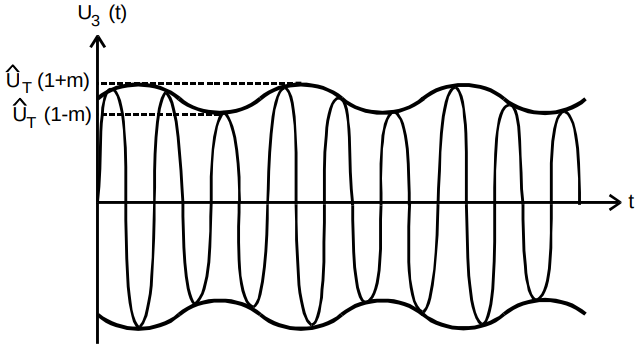
\includegraphics[width=0.55\textwidth]{ressources/T1.png}
    \caption{Darstellung einer amplitudenmodulierten Spannung in Abhängigkeit der Zeit $t$\cite{skript}.}
    \label{fig_T1}
\end{figure}

Um das Frequenzspektrum dieser Schwingung zu ermitteln, wird Gleichung \eqref{eq:1} mittels trigonometrischen Beziehungen zu
\begin{align}
	U(t)=\hat{U}_T\left(\cos{(\omega_Tt)+\frac{1}{2}m\cos{(\omega_T+\omega_M)t}}+\frac{1}{2}m\cos{(\omega_T-\omega_M)t})\right)
\end{align}
vereinfacht. Somit besteht das Frequenzspektrum aus den drei Frequenzen
\begin{align}
	\omega_T-\omega_M,\quad\omega,\quad\omega_T+\omega_M\;.
\end{align}
In Abbildung \ref{fig_T2} sind die zuvor beschriebenen Kreisfrequenzen gegen die Spannung aufgetragen.

\begin{figure}
    \centering
    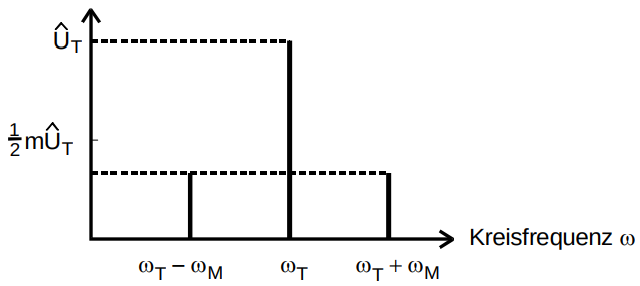
\includegraphics[width=0.55\textwidth]{ressources/T2.png}
    \caption{Darstellung eines Frequenzspektrums einer amplitudenmodulierten Spannung\cite{skript}.}
    \label{fig_T2}
\end{figure}

Bei der Betrachtung des Spektrums ist zu beachten, dass, wie auch in Abbildung \ref{fig_T2} zu sehen, die äußeren beiden Frequenzen, die sogenannten Seitenbänder, identische Informationen enthalten. Im Gegensatz dazu enthält die Frequenz $\omega_T$, die sogenannte Trägerabstrahlung, durch die fehlende Abhängigkeit von $\omega_M$ keine Information. Besteht der Umstand, dass $\omega_M$ nicht nur aus einer sondern aus einer Kombination mehrerer Frequenzen besteht, verbreitern sich die Seitenbänder in Abbildung \ref{fig_T2}. Nachteile der Amplitudenmodulation sind unter anderem die geringe Störsicherheit und die geringe Verzerrungsfreiheit. Beispielsweise kann es in engen Schaltkreise mit mangelnder Abschirmung zur Induktion einer Fremdspannung kommen, wodurch die Amplitude der Modulation beeinflusst wird. Unbeeinflusst bleibt die Frequenz, weshalb im Folgenden die Frequenzmodulation beschrieben wird.

\subsection{Frequenzmodulation}
\label{sec:Frequenzmodulation}
Bei der Frequenzmodulation entsteht eine Änderung der Trägerfrequenz verursacht durch ein Modulationssignal. Dabei ist zu betonen, dass nur die Frequenz eine Variation erfährt und die Amplitude konstant bleibt. Die modulierte Spannung kann wie folgt dargestellt werden:
\begin{align}
	U(t)=\hat{U}\sin{\left(\omega_Tt+m\frac{\omega_T}{\omega_M}\cos{(\omega_Mt)}\right)}
	\label{eq:2}
\end{align}
Die Momentanfrequenz wird dabei beschrieben durch
\begin{align}
	f(t)=\frac{\omega_T}{2\pi}(1-m\sin{(\omega_Mt)})\;.
\end{align}
Mit dem Frequenzhub
\begin{align}
	\Delta f=\frac{m\omega_T}{2\pi}
\end{align}
wird die Variationsbreite, also ein Maß für die Variation der Frequenz definiert. In Abbildung \ref{fig_T3} ist beispielhaft eine Frequenzmodulierte Schwingung skizziert.

\begin{figure}
    \centering
    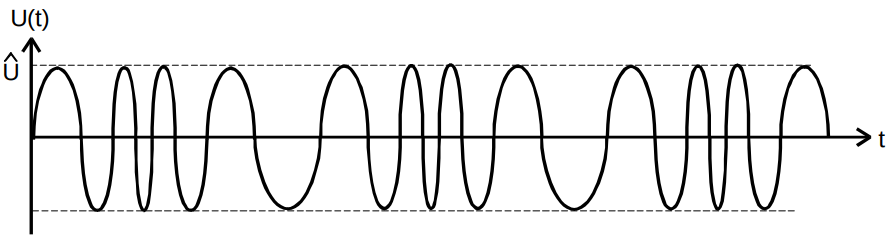
\includegraphics[width=0.85\textwidth]{ressources/T3.png}
    \caption{Darstellung einer frequenzmodulierten Spannung in Abhängigkeit der Zeit $t$\cite{skript}.}
    \label{fig_T3}
\end{figure}

Anhand einer sogenannten Schmalband-Frequenzmodulation, bei der gilt 
\begin{align}
	m\frac{\omega_T}{\omega_M}<<1,
\end{align}
soll im folgende grundlegende Eigenschaften der Frequenzmodulation verdeutlicht werden. Mittels trigonometrischer Funktionen wird Gleichung \eqref{eq:2} umgeformt zu
\begin{align}
	U(t)=\hat{U}\left(\sin{(\omega_Tt)}\cos{\left(m\frac{\omega_T}{\omega_M}\cos{(\omega_Mt)}\right)} + \cos{(\omega_Tt)}\sin{\left(m\frac{\omega_T}{\omega_M}\cos{(\omega_Mt)}\right)}\right) \:.
\end{align}
Mit einer Reihenentwicklung der Sinus- und Cosinustherme, bei der nur Therme erster Ordnung betrachtet werden, entsteht die folgende Gleichung
\begin{align}
	U(t)=\hat{U}\left(\sin{(\omega_Tt)+\frac{1}{2}m\frac{\omega_T}{\omega_M}\cos{(\omega_T+\omega_M)t}}+\frac{1}{2}m\frac{\omega_T}{\omega_M}\cos{(\omega_T-\omega_M)t})\right)\;,
\end{align}
die sehr große Ähnlichkeit zur amplitudenmodulierten Spannung aufweist, da auch hier das Frequenzspektrum aus den drei Frequenzen
\begin{align}
	\omega_T-\omega_M,\quad\omega,\quad\omega_T+\omega_M\;
\end{align}
besteht. Der wesentliche Unterschied besteht jedoch in der Trägerschwingung, da diese durch den Sinus um $90^{\circ}\text{C}$ Phasenverschoben wird.
Unter Berücksichtigung höherer Therme in der Reihenentwicklung ergibt sich 
\begin{align}
	U(t)=\hat{U}\sum_{n=-\infty}^{\infty} J_n\left(m\frac{\omega_T}{\omega_M}\right)\sin{(\omega_T+n\omega_M)}t\;. 
	\label{eq:3}
\end{align}
Der Ausdruck $J_n(x)$ steht dabei für die Besselfunktion n-ter Ordnung. Bei der Betrachtung von Gleichung \eqref{eq:3} fällt auf, dass der Iterator der Summe in der Sinusfunktion ein beliebig großes Frequenzspektrum ermöglicht. Da jedoch die Besselfunktion für steigende $n$ gegen Null strebt müssen nur Frequenzen nahe der Trägerfrequenz $\omega_T$ berücksichtigt werden.


% 2x2 Plot
% \begin{figure*}
%     \centering
%     \begin{subfigure}[b]{0.475\textwidth}
%         \centering
%         \includegraphics[width=\textwidth]{Abbildungen/Schaltung1.pdf}
%         \caption[]%
%         {{\small Schaltung 1.}}
%         \label{fig:Schaltung1}
%     \end{subfigure}
%     \hfill
%     \begin{subfigure}[b]{0.475\textwidth}
%         \centering
%         \includegraphics[width=\textwidth]{Abbildungen/Schaltung2.pdf}
%         \caption[]%
%         {{\small Schaltung 2.}}
%         \label{fig:Schaltung2}
%     \end{subfigure}
%     \vskip\baselineskip
%     \begin{subfigure}[b]{0.475\textwidth}
%         \centering
%         \includegraphics[width=\textwidth]{Abbildungen/Schaltung4.pdf}    % Zahlen vertauscht ... -.-
%         \caption[]%
%         {{\small Schaltung 3.}}
%         \label{fig:Schaltung3}
%     \end{subfigure}
%     \quad
%     \begin{subfigure}[b]{0.475\textwidth}
%         \centering
%         \includegraphics[width=\textwidth]{Abbildungen/Schaltung3.pdf}
%         \caption[]%
%         {{\small Schaltung 4.}}
%         \label{fig:Schaltung4}
%     \end{subfigure}
%     \caption[]
%     {Ersatzschaltbilder der verschiedenen Teilaufgaben.}
%     \label{fig:Schaltungen}
% \end{figure*}

\clearpage
\newpage
\section{Fehlerrechnung}
Dieses Kapitel listet kurz und bündig die benötigten und aus den Methoden der Statistik bekannten Formeln für die Fehlerrechnung auf.
Die Schätzung der Standardabweichung ist
\begin{equation}
  \label{eq:std}
  \Delta X = \sqrt{\frac{1}{n-1}\sum_{i=1}^n(X_i-\overline{X})^2}     \; .
\end{equation}
Der Mittelwert ist
\begin{equation}
  \overline{X} = \frac{1}{n} \sum_{i=1}^nX_i
\end{equation}
Der Fehler des Mittelwertes ist
\begin{equation}
  \label{eq:std_mean}
  \Delta \overline{X} = \sqrt{\frac{1}{n(n-1)}\sum_{i=1}^n(X_i-\overline{X})^2}   \; .
\end{equation}
Für fehlerbehaftete Größen, die auch in folgenden Formeln verwendet werden, muss die Fehlerfortpflanzung nach Gauß berücksichtigt werden.
\begin{equation}
  \label{eq:GFFP}
  \Delta f = \sqrt{\sum_{i=1}^n \left(\frac{\partial f}{\partial X_i}\right)^2 \cdot (\Delta X_i)^2}
\end{equation}
Bei der linearen Regressionsrechnung sind die Parameter $m$ und $b$ der Ausgleichsgerade $y=mx+b$ wie folgt gegeben:
\begin{align}
  m &= \frac{\overline{xy}-\overline{x}\cdot\overline{y}}{\overline{x²} - \overline{x}²} & &  b = \overline{y} - m \overline{x}  \; .
\end{align}
Dabei sind $x_i$ und $y_i$ linear abhängige Messgrößen. Der Fehler dieser Parameter wiederum errechnet sich aus
\begin{align}
  \sigma_m^2 &= \frac{\sigma^2}{n(\overline{x²} - \overline{x}²)} & &\sigma_b^2 = \frac{\sigma^2\overline{x²}}{n(\overline{x²} - \overline{x}²)} \; .
\end{align}
Relative Abweichungen einer Messgröße $x$ gegenüber Literaturwerten $x_\text{Lit}$ werden nach der Vorschrift
\begin{align}
  R_x = \frac{x-x_\text{Lit}}{x_\text{Lit}}
\end{align}
berechnet.
% Wenn Messdaten mit Vorhersagen verglichen werden sollen, benutzt man häufig die \emph{root mean square deviation}. Diese ist gegeben durch
% \begin{equation}
%   \label{eq:RMSE}
%   \textrm{RMSD} = \sqrt{\overline{(Y_\textrm{Messung}-Y_\textrm{Vorhersage})^2}}  \; .
% \end{equation}

\clearpage
\newpage
\section{Versuchsaufbau}
\label{sec:Versuchaufbau}
In diesem Kapitel werden alle in diesem Versuch verwendeten elektronischen Schaltungen für die Modulation als auch die Demodulation beschrieben und erläutert.
\subsection{Modulation}
\subsubsection{Primitive Modulatorschaltung mittels Diode}
\label{sec:Primitive_Modulatorschaltung_mittels_Diode}
Zur Realisierung einer Amplitudenmodulation wird eine Schaltung benötigt, die die Trägerspannung mit der Modulationsspannung multipliziert. Eine solcher Aufbau ist in Abbildung \ref{fig_10} dargestellt.

\begin{figure}
    \centering
    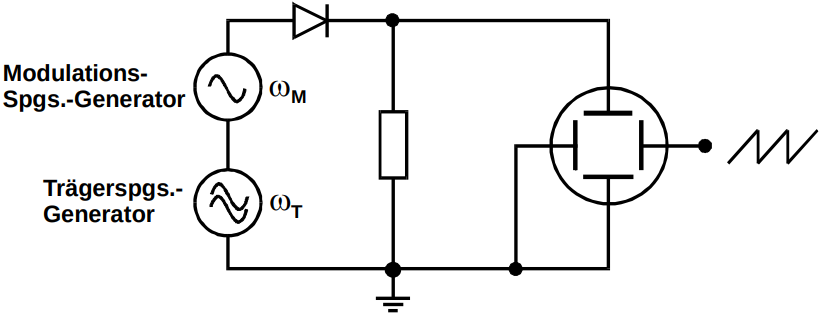
\includegraphics[width=0.55\textwidth]{ressources/A10.png}
    \caption{Aufbau einer Modulatorschaltung mittels Diode\cite{skript}.}
    \label{fig_10}
\end{figure}

Durch die nicht lineare Diodenkennlinie entstehen während der Multiplikation durch die Potenzreihenentwicklung neben dem benötigten Term $U_T \cdot U_M$ im zweiten Glied auch unerwünschte Therme höherer Ordnung der Träger- und Modulationsspannung. Dessen Frequenzen liegen außerhalb des Intervalls $[\omega_T-\omega_M, \omega_T+\omega_M]$ und können somit durch Bandfilter unterdrückt werden.

\subsubsection{Ringmodulator}
\label{sec:Ringmodulator}
Durch den sogenannten Ringmodulator, siehe Abbildung \ref{fig_02}, werden die bei der Schaltung im vorherigen Kapitel unerwünscht entstandenen Komponenten vermieden. Wie in Abbildung \ref{fig_02} dargestellt, sind die vier Dioden der Hauptbestandteil der Schaltung. 

\begin{figure}
    \centering
    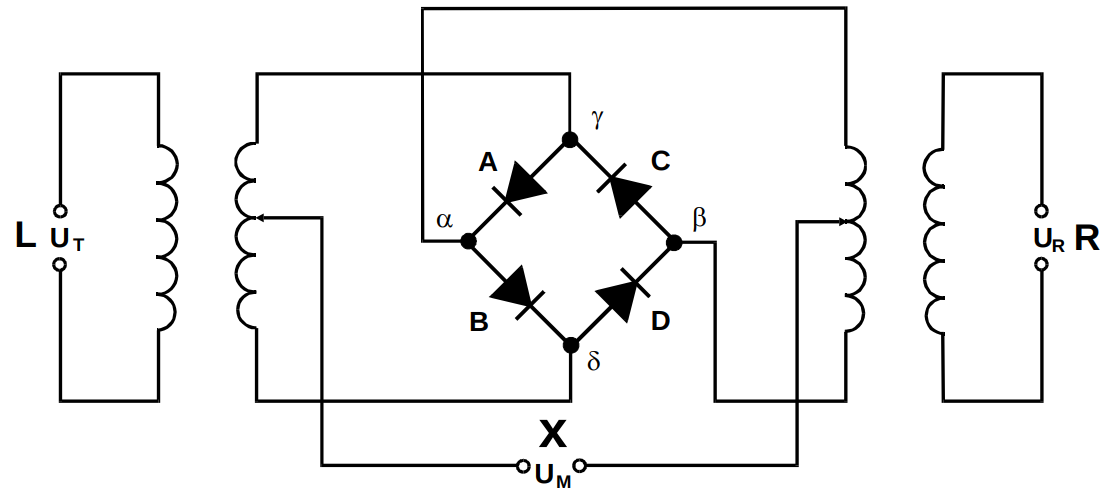
\includegraphics[width=0.55\textwidth]{ressources/A2.png}
    \caption{Aufbau eines Ringmodulatorschaltung \cite{skript}.}
    \label{fig_02}
\end{figure}

Durch diese wird eine Spannungsteiler an den Punkten $\alpha$ und $\beta$ realisiert, wodurch, bei baugleichen Dioden und ohne anliegender Modulationsspannung, keine Potentialdifferenz zwischen dem beiden besagten Punkten auftritt. Erst durch das Anlegen einer Modulationsspannung $U_M$ wird das Gleichgewicht gestört und die Teilungsverhältnisse der Dioden schwingen im Rhythmus von $U_M(t)$. Bei idealen Verhältnissen ist somit das Produkt der Eingangsspannungen proportional zur Ausgangsspannung. Aus diesem Grund entsteht bei dem Ringmodulator keine Trägerabstrahlung, weshalb nur die Seitenbänder entstehen.

\subsubsection{Frequenzmodulator mit geringem Frequenzhub}
\label{sec:Frequenzmodulator_mit_geringem_Frequenzhub}
Grundlage ist hierfür der in Kapitel \ref{sec:Ringmodulator} beschriebene Ringmodulator. Da durch diesen nur die Seitenbändern ohne Trägerabstrahlung erzeugt werden, muss die Trägerfrequenz mit einer Phasenverschiebung von $\pi/2$ gesondert hinzugefügt werden. Dieses wird, wie in Abbildung \ref{fig_03} dargestellt, über ein Laufzeitkabel von $\SI{250}{\ns}$ realisiert. 

\begin{figure}
    \centering
    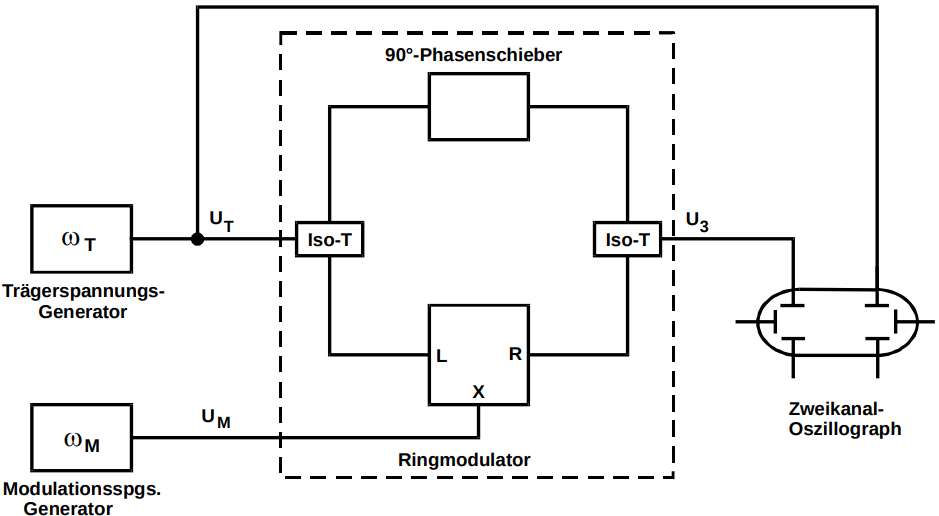
\includegraphics[width=0.55\textwidth]{ressources/A3.png}
    \caption{Darstellung einer Frequenzmodulatorschaltung mit Laufzeitkabel \cite{skript}.}
    \label{fig_03}
\end{figure}

Um die gewünschte Phasenverschiebung zu erhalten, kann über die zuvor passend eingestellte Periodendauer die benötigte Frequenz bestimmt werden.

\subsubsection{Phasenempfindlichkeit des Ringmodulators}
\label{sec:Phasenempfindlichkeit_der_Gleichrichterdiode}
Mit der folgenden Schaltung in Abbildung \ref{fig_11} wird durch die Variation der Frequenz und einem Laufzeitkabel die Phasenverschiebung erzeugt. 
\begin{figure}
    \centering
    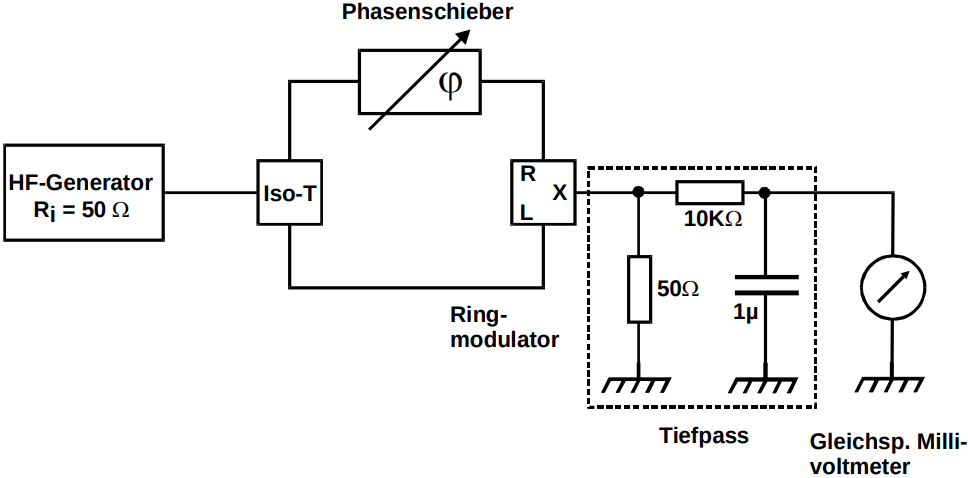
\includegraphics[width=0.55\textwidth]{ressources/A11.png}
    \caption{Darstellung einer Ringdiodenschaltung in Verbindung mit einem Laufzeitkabel und einem Amperemeter zu Überprüfung der Phasendifferenz \cite{skript}.}
    \label{fig_11}
\end{figure}
Über das Voltmeter wird die Spannung in Abhängigkeit der Frequenz dargestellt, wodurch die Proportionalität $U\approx\cos{(\phi)}$ überprüft wird. Hierfür wird die Abhängigkeit der Phase von der Frequenz verwendet.

\subsection{Demodulation}

\subsubsection{Demodulation amplitudenmodulierter Schwingungen}
\label{sec:Demodulation_amplitudenmodulieter_Schwingungen}
Zur Demodulation wird ebenfalls ein Ringmodulator verwendet. Wie in Abbildung \ref{fig_04} dargestellt, ist am Eingang L die modulierte Spannung und am Eingang R die Trägerspannung angelegt. 

\begin{figure}
    \centering
    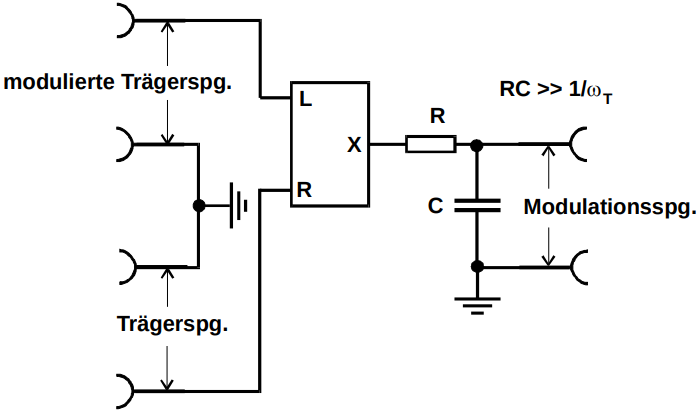
\includegraphics[width=0.55\textwidth]{ressources/A4.png}
    \caption{Darstellung eines Ringmodulators zur Demodulation einer amplitudenmodulierten Schwingung \cite{skript}.}
    \label{fig_04}
\end{figure}

Da die Frequenzen der Eingänge addiert und subtrahiert werden, ergeben sich aus den angelegten Frequenzen $\omega_T\pm\omega_M$ (Eingang L) und $\omega_T$ (Eingang R) am Ausgang X die Frequenzen $2\omega_T\pm\omega_M$ und $\omega_M$.

\subsubsection{Demodulator-Schaltung mit einer Gleichrichter-Diode}
\label{DSmeGD}
Ein weiteres Verfahren zur Demodulation einer Amplitudenmodulation besteht in der Verwendung einer Gleichrichterdiode mit geeignetem Tiefpass. Diese Schaltung findet Anwendung, wenn die ursprüngliche Trägerspannung nicht zur Demodulation zur Verfügung steht. Wie in Abbildung \ref{fig_05} dargestellt, werden durch die Diode sämtliche negativen Halbwellen der Signalspannung entfernt.

\begin{figure}
    \centering
    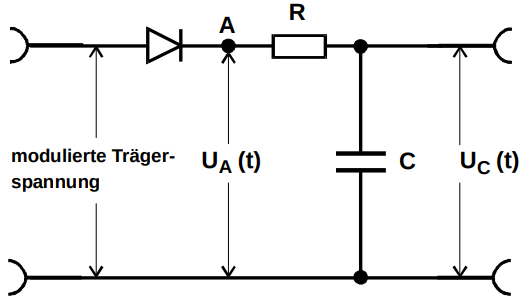
\includegraphics[width=0.55\textwidth]{ressources/A5.png}
    \caption{Darstellung einer Demodulationsschaltung mit Hilfe einer Gleichrichterdiode \cite{skript}.}
    \label{fig_05}
\end{figure}

Die in Abbildung \ref{fig_06} dargestellte Spannung am Punkt A enthält zu diesem Zeitpunkt hochfrequente Anteile der Form $\omega_T$, $2\omega_T$, $4\omega_T$ u.s.w. und $\omega_M$. Da die Beziehung $\omega_T>>\omega_M$ weiterhin gilt, kann die hohe Trägerfrequenz und deren Vielfache durch einen Tiefpass unterdrückt werden, sodass die in Abbildung \ref{fig_07} dargestellte Modulationsfrequenz extrahiert werden kann. 

\begin{figure}
    \centering
    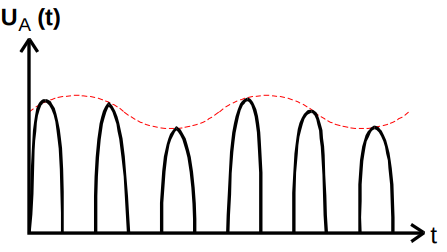
\includegraphics[width=0.45\textwidth]{ressources/A6.png}
    \caption{Darstellung der Spannung am Punkt A der Schaltung \ref{fig_05} \cite{skript}.}
    \label{fig_06}
\end{figure}

\begin{figure}
    \centering
    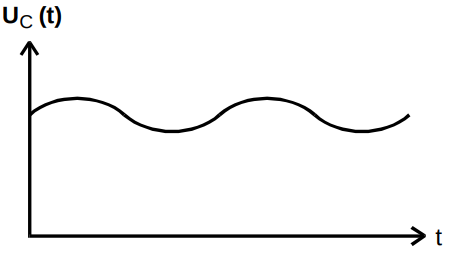
\includegraphics[width=0.45\textwidth]{ressources/A7.png}
    \caption{Darstellung der Spannung nach dem Tiefpass der Schaltung \ref{fig_05} \cite{skript}.}
    \label{fig_07}
\end{figure}

In der Realität ist die erhaltene Frequenz jedoch gegenüber der ursprünglichen Modulationsfrequenz verzerrt, da die Diode einen annähernd exponentiellen Kennlinienverlauf aufweist. Wird jedoch eine sehr kleine Modulationsfrequenz gewählt, kann die Kennlinie der Diode linear genähert werden und so eine Verzerrung vermindert werden.

\subsubsection{Demodulation frequenzmodulierter Schwingungen}
\label{sec:Demodulation_frequenzmodulieter_Schwingungen}
Im ersten Teil der Demodulation findet die Umwandlung in eine amplitudenmodulierte Schwingung statt. Dieses wird durch einen LC-Schwingkreis realisiert, wie in Abbildung \ref{fig_12} zu sehen. 

\begin{figure}
    \centering
    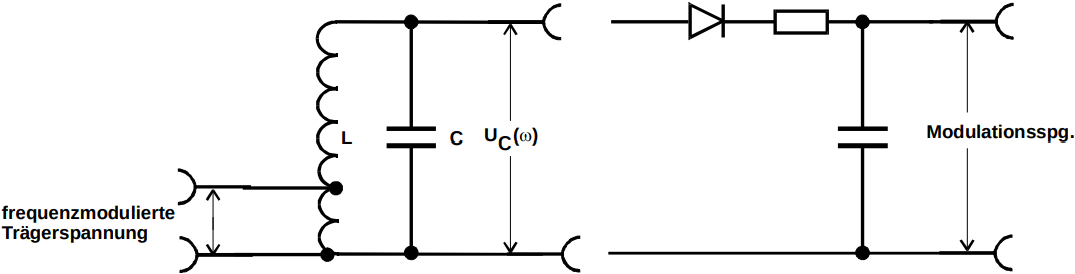
\includegraphics[width=0.80\textwidth]{ressources/A12.png}
    \caption{Darstellung eines LC-Schwingkreises mit dem die frequenzmodulierte Schwingung in eine amplitudenmodulierte Schwingung überführt wird. \cite{skript}.}
    \label{fig_12}
\end{figure}


Aus diesem Grund ist die Resonanzfrequenz der Schaltung so gewählt, dass die Trägerfrequenz und der Frequenzhub auf der Flanke der Resonanzkurve liegt (siehe Abbildung \ref{fig_08}). Ändert sich Momentanfrequenz der Schwingung, so entsteht am Ausgang der Schaltung eine hochfrequente Spannung, die keine konstante Amplitude mehr aufweist, sondern deren Amplitude im Rhythmus der Modulationsfrequenz schwingt. Im zweiten Schritt ist die Demodulation der amplitudenmodulierten Schwingung durch die in Kapitel \ref{sec:Demodulation_amplitudenmodulieter_Schwingungen} oder \ref{DSmeGD} vorgestellte Methoden durchzuführen. 

\begin{figure}
    \centering
    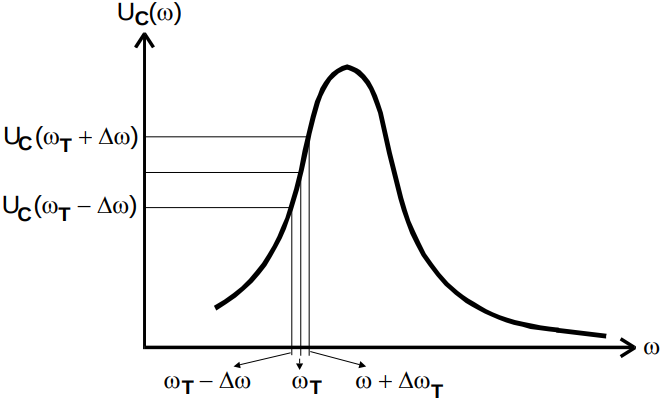
\includegraphics[width=0.55\textwidth]{ressources/A8.png}
    \caption{Darstellung der Resonanzkurve des LC-Schwingkreises und dem Frequenzspektrum der modulierten Schwingung auf dessen Flanke \cite{skript}.}
    \label{fig_08}
\end{figure}

\clearpage
\newpage
\section{Durchführung}
\label{sec:Durchführung}

\subsection{Amplitudenmodulierte Schwingungen}
Zu Beginn soll eine amplitudenmodulierte Schwingung erzeugt werden. Dafür werden die Trägerfrequenz $\omega_T$ und die Modulationsfrequenz $\omega_M$ sogewählt, dass die Trägerfrequenz etwa um einen Faktor 100 hochfrequenter ist als die Modulationsspannung. Für die anschließende Erzeugung wird ein Ringmodulator nach Kapitel XXX verwendet. Um die Korrektheit der amplitudenmodulierte Schwingungen zu überprüfen wird an einem weiteren Kanal des Oszilloskops zusätzlich die Modulationsfrequenz angelegt. Im folgenden wird das Frequenzspektrum mittels Frequenzanalysator untersucht und das Ergebniss von dem Bildschirm des Frequenzanalysators abfotographiert.
\\
Anschleißend wird die Erzeugung einer amplitudenmodulierten Schwingung mit der in Kapitel XXX vorgestellten Diodenschaltung untersucht. Dabei können die eingestellten Frequenzen beibehalten werden. Es wird ebenfalls mittels Frequenzanalysator das Spektrum untersucht und dokumentiert.

\subsection{Frequenzmodulierte Schwingungen}
Für die Erzeugung wird die in Kapitel XXX beschriebene Schaltung verwendet. Dabei muss auf die korrekte Phasenverschiebung, verursacht durch das Laufzeitkabels, geachtet werden. Mit einer gegebenen Periodendauer von $\SI{250}{\ns}$ ergibt sich die benötigte Frequnenz zu $\omega=\SI{1}{\mega\hertz}$. An dem Oszilloskop werden Einstellungen vorgenommen, sodass die Verschmierung der modulierten Spannung über eine Periode zu erkennen ist. Mit Hilfe der "Curser"-Funktion wird zusätzlich die maximale Breite in X-Richung der Verschmierung in mitten einer Periode bestimmt. Alles zwischenschritte werden dabei dokumentiert und das aufgenommene Frequenzspektrum am Frequenzanalysator fotographiert.

\subsection{Gleichrichtereigenschaften des Ringmodulators}
Mit der in Kapitel XXX beschriebenen Schaltung wird die Spannung in Anhängigkeit der Trägerfrequenz mit Hilfe eines Voltmeters vermessen. Die sich ergebende Proportionaltiät zum Cosinus der Phase $phi$ wird solange vermessen, bis die aufgenommenen Daten für eine volle Periode ausreichen.

\subsection{Demodulation einer amplitudenmodulierten Schwingung}
In diesem Abschnitt soll eine amplitudenmodulierte Schwingung demoduliert werden, mittels der in Kapitel XXX beschriebenen Schaltung. Erneut wird mit dem zweiten Kanal des Oszilloskops überprüft, ob demodulierte Schwinkung der ursprünglichen modulationsfrequenz übereinstimmt. Auch hier wird wieder anschließend das Frequenzspektrum mit Hilfe des Frequenzanalysator aufgezeichnet.
\\
Ebenfalls soll die amplitudenmodulierte Schwingung, die durch die Diodenschaltung nach Kapitel XXX erzeugt wurde, demoduliert werden. Hierzu wird die Schaltung aus Kapitel XXX verwendet. Diese Mal werden auch die Zwischenschritte(nach der Diode und nach dem Tiefpass) dokumentiert, sodass die einzelnen Vorgänge besser nachvollzogen werden können.

\subsection{Demodulation einer frequenzmodulierten Schwingung}
Als letztes soll die frequenzmodulierten Schwingung, durch den in Kapitel XXX beschrieben Aufbau demoduliert werden. Hierfür muss die Kapazität des Kondensator so gewählt werden, dass sich die Frequenzen der Seitenbänder auf der Flanke der Resonanzkurve befinden. Somit müsste eine amplitudenmodulierte Schwingung am Osziloskop messbar sein. Auch hier werden wieder die Teilschritte (nach der Diode und nach dem Tiefpass) genau dokumentiert. Schlussendlich wird erzeugte demodulierte Spannung mit der ursprünglichen Modulationspannung vergleichen. 
\clearpage
\newpage
\section{Auswertung}
\label{sec:Auswertung}
\subsection{Bestimmung des lokalen Erdmagnetfeld}
Für die Bestimmung des Erdmagnetfeldes werden die Magnetfeldstärken der
Sweepfeld- und Horizontalfeld in Abhängigkeit der Resonanzfrequenz gemessen.
Die gemessenen Messwerte werden in der Tabelle \ref{tabmess1} dargestellt.
 \begin{table}
   \centering
   \caption{Position der Resonanzstellen für verschiedene Frequenzen}
   \label{tabmess1}
   \sisetup{parse-numbers=false}
   \begin{tabular}{c|c|c|c|c}
     \toprule
    $f$ in Hz & Sweep 1& Horizontal 1 & Sweep 2&Horizontal 2 \\
     \midrule
     100 &  5.66 &  6.84  & 0   &   0   \\
     200 &  5.78 & 7.13  & 0.15 &  0.15  \\
     300 &  5.43 & 8.96  & 0.20 &  0.20 \\
     400 &  4.24 & 9.01  & 0.28 &  0.28 \\
     500 &  2.41 & 8.32  & 0.38 &  0.38 \\
     600 &  1.67 & 8.71  & 0.44 &  0.44 \\
     700 &  0.98 & 9.28  & 0.52 &  0.52 \\
     800 &  3.34 & 7.73  & 0.52 &  0.64 \\
     900 &  2.26 & 4.76  & 0.60 &  0.78 \\
     1000 & 4.10 & 6.01  & 0.61 &  0.83 \\
     \bottomrule
   \end{tabular}
 \end{table}




% Sämtliche im Folgenden durchgeführten Ausgleichsrechnungen werden mit der \emph{curve fit} Funktion aus dem für \emph{Python} geschriebenen package \emph{NumPy}\cite{scipy} durchgeführt. Fehlerrechnungen werden mit dem für \emph{Python} geschriebenen package \emph{Uncertainties}\cite{uncertainties} ausgeführt.

% % Examples
% \begin{equation}
%   U(t) = a \sin(b t + c) + d
% \end{equation}
%
% \begin{align}
%   a &= \input{build/a.tex} \\
%   b &= \input{build/b.tex} \\
%   c &= \input{build/c.tex} \\
%   d &= \input{build/d.tex} .
% \end{align}
% Die Messdaten und das Ergebnis des Fits sind in Abbildung~\ref{fig:plot} geplottet.
%
% %Tabelle mit Messdaten
% \begin{table}
%   \centering
%   \caption{Messdaten.}
%   \label{tab:data}
%   \sisetup{parse-numbers=false}
%   \begin{tabular}{
% % format 1.3 bedeutet eine Stelle vorm Komma, 3 danach
%     S[table-format=1.3]
%     S[table-format=-1.2]
%     @{${}\pm{}$}
%     S[table-format=1.2]
%     @{\hspace*{3em}\hspace*{\tabcolsep}}
%     S[table-format=1.3]
%     S[table-format=-1.2]
%     @{${}\pm{}$}
%     S[table-format=1.2]
%   }
%     \toprule
%     {$t \:/\: \si{\milli\second}$} & \multicolumn{2}{c}{$U \:/\: \si{\kilo\volt}$\hspace*{3em}} &
%     {$t \:/\: \si{\milli\second}$} & \multicolumn{2}{c}{$U \:/\: \si{\kilo\volt}$} \\
%     \midrule
%     \input{build/table.tex}
%     \bottomrule
%   \end{tabular}
% \end{table}
%
% % Standard Plot
% \begin{figure}
%   \centering
%   \includegraphics{build/plot.pdf}
%   \caption{Messdaten und Fitergebnis.}
%   \label{fig:plot}
% \end{figure}
%
% 2x2 Plot
% \begin{figure*}
%     \centering
%     \begin{subfigure}[b]{0.475\textwidth}
%         \centering
%         \includegraphics[width=\textwidth]{Abbildungen/Schaltung1.pdf}
%         \caption[]%
%         {{\small Schaltung 1.}}
%         \label{fig:Schaltung1}
%     \end{subfigure}
%     \hfill
%     \begin{subfigure}[b]{0.475\textwidth}
%         \centering
%         \includegraphics[width=\textwidth]{Abbildungen/Schaltung2.pdf}
%         \caption[]%
%         {{\small Schaltung 2.}}
%         \label{fig:Schaltung2}
%     \end{subfigure}
%     \vskip\baselineskip
%     \begin{subfigure}[b]{0.475\textwidth}
%         \centering
%         \includegraphics[width=\textwidth]{Abbildungen/Schaltung4.pdf}    % Zahlen vertauscht ... -.-
%         \caption[]%
%         {{\small Schaltung 3.}}
%         \label{fig:Schaltung3}
%     \end{subfigure}
%     \quad
%     \begin{subfigure}[b]{0.475\textwidth}
%         \centering
%         \includegraphics[width=\textwidth]{Abbildungen/Schaltung3.pdf}
%         \caption[]%
%         {{\small Schaltung 4.}}
%         \label{fig:Schaltung4}
%     \end{subfigure}
%     \caption[]
%     {Ersatzschaltbilder der verschiedenen Teilaufgaben.}
%     \label{fig:Schaltungen}
% \end{figure*}

\clearpage
\newpage
\section{Diskussion}
\label{sec:Diskussion}
Die transversal und longitudinal Komopnente der Relaxationszeit konnten
mit kleinen Fehler bestimmt werden:
$$(T_1=2.1 \pm 0.2 \,)\, \text{s} \quad \quad T_2=1.4 \pm 0.2 \,)\, \text{s}$$
Die Messwerte weisen eine gute Übereinstimmung, bis ein
einzelne Ausreißer, mit den Fit auf.\\
Der bestimmte Feldgradient $G=-0.41$ liegt unter dem erwarteten Wert,
von $\approx G=-1\,\text{T}\text{m}^{-1}$. Sodass die damit bestimmte
Diffusionskonstante große Abweichungen $\approx 53\, \%$ vom Literaturwert $D_\text{lit}=2.1\cdot
10^{-9}\,\text{m}^2\text{s}^{-1}$\cite{diff}.\\
Der Verlgeich der bestimmten Viskosität $(\eta=0.949)\,$mPa$\,$s
mit dem Theoriewert $(\eta=0.890)\,$mPa$\,$s \cite{visko} zeigt eine Abweichung von $\approx
18\,\%$ eine leichte Abweichung.\\
Der berechnete Radius des Wassermolekühls $(1.7 \pm 0.6)\cdot 10^{-11},$m
lässt sich mit einer Abschätzung zum Molekühlradius,
welche nur von der Dichte, dem Molekulargewicht $m=18.01528\,$g/mol \cite{visko}
und der Annahme der dichten kexagonalen Kugelpackung abhängt. Für
die dichte Kugelpackung wird $n=74\%$ verwendet, es ergibt sich für
die Abschätzung des Molekülradius:
$$R=\left( \frac{3m}{4\pi \rho \cdot 0.74}\right)^{1/3}\approx 2.13\cdot 10^{-11}\,\text{m}$$
Der berechnete Wert und die Abschätzung des Radius $R$ weißen eine
Größenordnung Unterschied auf. Diese könnte auf sich durch die
ungenauen Werte für die Diffusionskonstante und auf den Feldgradienten
zurückführen lassen. Des Weiteren wird hier nur eine Abschätzung des Radius
$R$ vorgenommen. Dennoch sollte das Ergebnis in der selben
Größenordnung liegen.

\clearpage
\newpage

\printbibliography

\clearpage
\newpage
% % % \begin{appendix}
% % % \section{Messdaten}
% % % \centering
% % % \begin{figure}
% % % \includepdf[width=0.9\textwidth, pages={1}]{Bilder/Messdaten.pdf}
% % % \end{figure}
% % % \newpage
% % % \begin{figure}
% % % \includepdf[width=0.9\textwidth, pages={2}]{Bilder/Messdaten.pdf}
% % % \end{figure}
% % %
% % % \end{appendix},


% % % % Standard Plot
% \begin{figure}
%   \centering
%   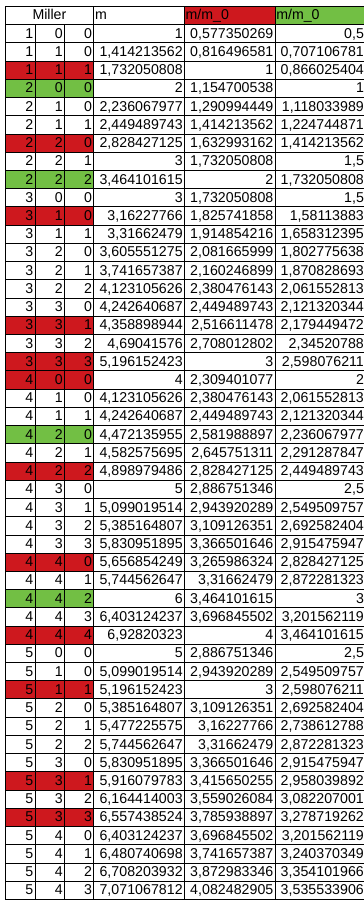
\includegraphics{ressources/Steinsalz.png}
%   \caption{Millerindizes und das theoretische Verhältnis nach \ref{eq:dm} für die Steinsalz/Fluorit-Struktur (a). Die grün hinterlegten Felder stellen schwache und die rot hinterlegten Felder starke Reflexe dar.}
%   \label{fig:Anhang1}
% \end{figure}

% \begin{figure}
%   \centering
%   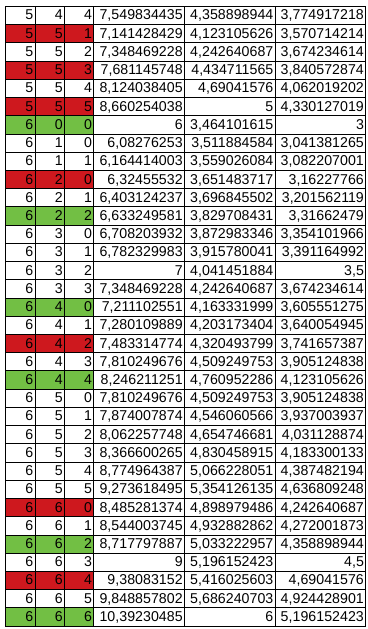
\includegraphics{ressources/Steinsalz2.png}
%   \caption{Millerindizes für die Steinsalz/Fluorit-Struktur (b).}
%   \label{fig:Anhang2}
% \end{figure}

% \begin{figure}
%   \centering
%   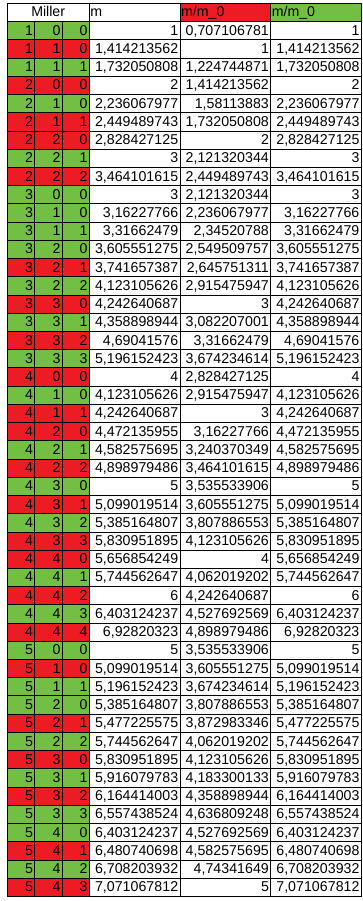
\includegraphics{ressources/Caesium.png}
%   \caption{Millerindizes und das theoretische Verhältnis nach \ref{eq:dm} für die Caesium-Struktur (a). Die grün hinterlegten Felder stellen schwache und die rot hinterlegten Felder starke Reflexe dar.}
%   \label{fig:Anhang3}
% \end{figure}

% \begin{figure}
%   \centering
%   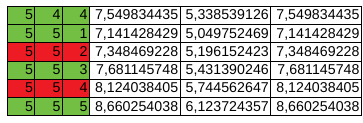
\includegraphics{ressources/Caesium2.png}
%   \caption{Millerindizes für die Caesium-Struktur (b).}
%   \label{fig:Anhang4}
% \end{figure}

% \begin{figure}
%   \centering
%   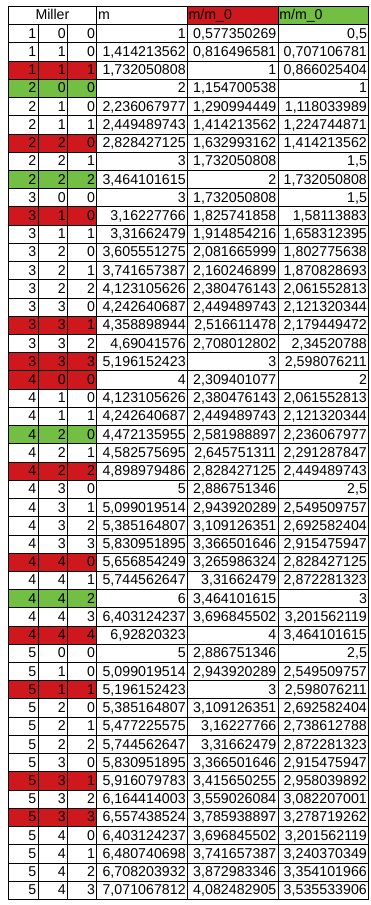
\includegraphics{ressources/Zinkblende.png}
%   \caption{Millerindizes und das theoretische Verhältnis nach \ref{eq:dm} für die Zinkblende-Struktur (a). Die grün hinterlegten Felder stellen schwache und die rot hinterlegten Felder starke Reflexe dar.}
%   \label{fig:Anhang5}
% \end{figure}

% \begin{figure}
%   \centering
%   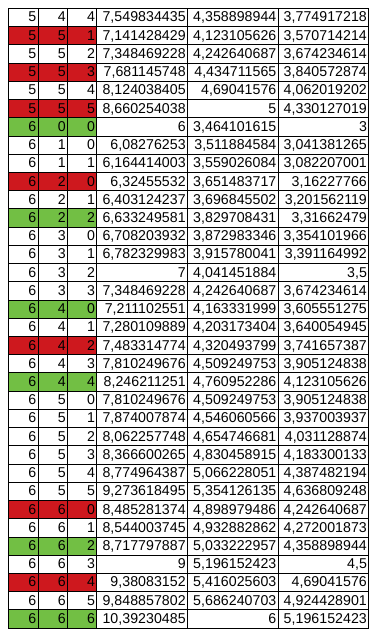
\includegraphics{ressources/Zinkblende2.png}
%   \caption{Millerindizes für die Zinblenden-Struktur (b).}
%   \label{fig:Anhang6}
% \end{figure}

\end{document}


% % Examples
% \begin{equation}
%   U(t) = a \sin(b t + c) + d
% \end{equation}
%
% \begin{align}
%   a &= \input{a.tex} \\
%   b &= \input{b.tex} \\
%   c &= \input{c.tex} \\
%   d &= \input{d.tex} .
% \end{align}
% Die Messdaten und das Ergebnis des Fits sind in Abbildung~\ref{fig:plot} geplottet.
%
% %Tabelle mit Messdaten
% \begin{table}
%   \centering
%   \caption{Messdaten.}
%   \label{tab:data}
%   \sisetup{parse-numbers=false}
%   \begin{tabular}{
%     S[table-format=1.3]
%     S[table-format=-1.2]
%     @{${}\pm{}$}
%     S[table-format=1.2]
%     @{\hspace*{3em}\hspace*{\tabcolsep}}
%     S[table-format=1.3]
%     S[table-format=-1.2]
%     @{${}\pm{}$}
%     S[table-format=1.2]
%   }
%     \toprule
%     {$t \:/\: \si{\milli\second}$} & \multicolumn{2}{c}{$U \:/\: \si{\kilo\volt}$\hspace*{3em}} &
%     {$t \:/\: \si{\milli\second}$} & \multicolumn{2}{c}{$U \:/\: \si{\kilo\volt}$} \\
%     \midrule
%     \input{table.tex}
%     \bottomrule
%   \end{tabular}
% \end{table}
%
% % Standard Plot
% \begin{figure}
%   \centering
%   \includegraphics{plot.pdf}
%   \caption{Messdaten und Fitergebnis.}
%   \label{fig:plot}
% \end{figure}
